\begin{figure}
    \centering
    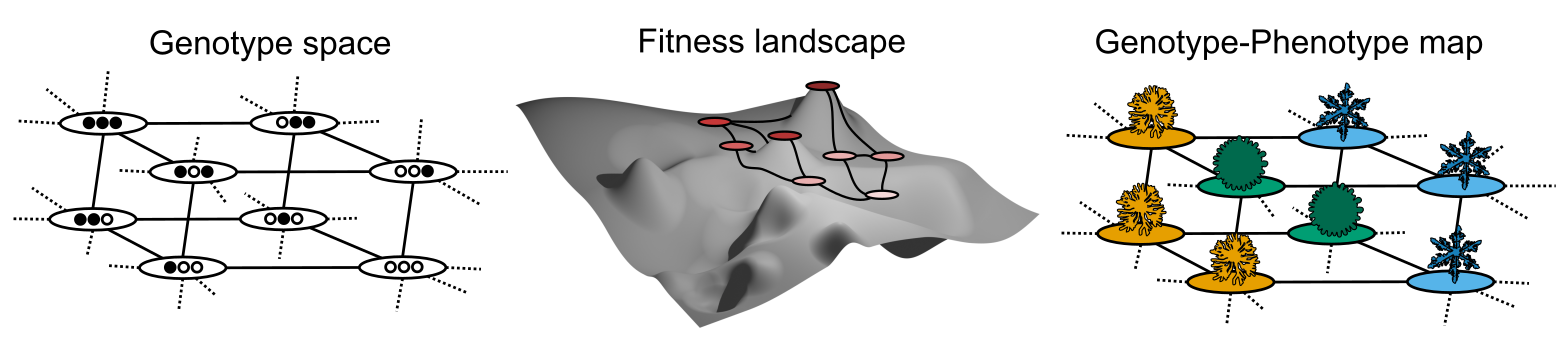
\includegraphics[width=1.0\linewidth]{img/fitness_landscapes.png}
    \caption{\textbf{Three flavors of biological genetic spaces}. The \textit{genotype space} (left) is a network of genotypes, with edges connecting genotypes that differ by a single mutation. A subset of a much larger genotype space is shown here, consisting of two alternative allelic states ($K=2$, filled or open circle) at three sites ($N=3$). A \textit{fitness landscape} (middle) is induced on this space when each genotype is assigned a value denoting its reproductive success in an environment. One may draw this landscape with the fitness values along a third dimension. However, this visualization only works for 2-dimensional genotype spaces, which are rare (if not absent) in biological systems. Even the simple genotype space shown here cannot be drawn as a planar network. Alternatively, the genotypes may be assigned ``phenotypes'' that denote the visible characteristics of the resulting organisms (e.g., colony morphology of a bacterium). This mapping of genotypes to phenotypes on an existing genotype-space forms the \textit{genotype-phenotype map} (right).}
    \label{fig:fitness_landscapes}
\end{figure}
